\section{Introduction}

The most studied algorithm in \acrfullPl{msr} is the self-reconfiguration algorithm which causes the modules to move from one configuration (the \textit{initial shape}) to another (the \textit{goal shape}) (see Figure~\ref{fig:reconfiguration:example-car}). 

\begin{figure}[!h]
	\centering
	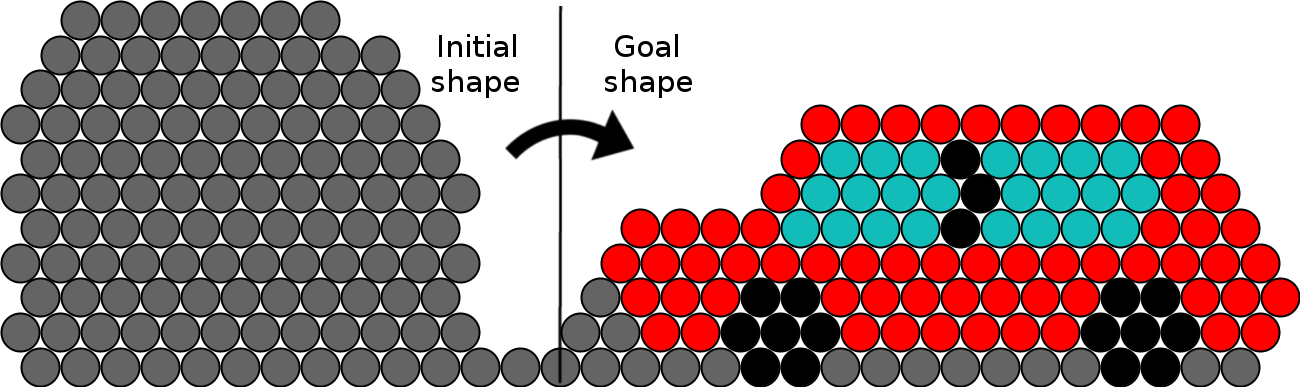
\includegraphics[width=0.7\linewidth]{images/reconfiguration/car}
	\caption{Example of initial and goal shapes. Self-reconfiguration is the process during which the initial clump of modules on the left self-reconfigures into the car shape on the right.}
	\label{fig:reconfiguration:example-car}
\end{figure}

As explained in the Introduction chapter, self-reconfiguration algorithms pose several algorithmic challenges. In the first place, planning is challenging as the number of possible unique configurations is huge and the exploration space between two random configurations is exponential in the number of modules, due to potential concurrent moves. This prevents us from finding a complete optimal planning for all but the simplest configurations. In addition to the path-planning problem, the distributed coordination of mobile autonomous modules connected in time-varying ways is also a challenging issue. In particular, modules have to coordinate their motions in order not to collide with each other.

Self-reconfiguration algorithms are tailored for a specific class of modular robots, with specific motion constraints~\cite{stoy2011current}, for example using cubes sliding on the floor, some motions need a cooperation process that complicates motion algorithms~\cite{pb16:ip}. In this work, we consider the 2D Catoms (see Chapter~\ref{chapter:context}). Our assumptions and system model are detailed in Section~\ref{section:reconfiguration:model}).

The contribution of this chapter is to propose the Cylindrical-Catoms Self-Reconfiguration (C2SR) algorithm\footnote{Some simulations of self-reconfiguration with C2SR are available online in video at \url{https://youtu.be/XGnY-oS4Nw0}} which is asynchronous, deterministic, fully decentralized and able to manage almost any kind of initial and goal compact shapes (see Section~\ref{section:reconfiguration:at-a-glance}). Although our work is focused on the algorithm, we carry out our analysis with respect to the hardware constraints of the 2D Catoms. C2SR is inspired by the algorithm in~\cite{rubenstein2014programmable} proposed for swarm robotic systems which assume different physical constraints. C2SR is a step toward realizing programmable matter.

We implemented our algorithm and evaluated it through simulations with VisibleSim. We show the effectiveness of C2SR on large-scale ensembles composed of up to ten thousand modules. We also show the effectiveness of our algorithm and study its performance in terms of communications, movements, and execution time.

The rest of this chapter is organized as follows. In section~\ref{section:reconfiguration:model}, we define the system model and assumptions. Afterwards, we discuss the related work in section~\ref{section:reconfiguration:related-work}. In section~\ref{section:reconfiguration:at-a-glance}, we present the general idea of C2SR and in section~\ref{section:reconfiguration:algorithm}, we describe its implementation. In section~\ref{section:reconfiguration:evaluation}, experimental results are presented and analyzed. Section~\ref{section:reconfiguration:conclusion} concludes this chapter. 

\section{System Model and Assumptions}
\label{section:reconfiguration:model}

In this chapter, we consider the 2D Catoms. This section presents our assumptions and system model.

We assume that 2D Catoms are organized in a horizontal pointy-topped hexagonal lattice where modules have up to six neighbors. Modules can communicate together using neighbor-to-neighbor communications. We assume that modules automatically discover their neighbors, using communications after becoming attached. We consider that moving modules cannot communicate with any other module. $\mathcal{N}^{N}_{C_i}$ denotes the network neighbors of the module $C_i$. Catoms on the periphery have \acrfull{cw} and \acrfull{ccw} neighboring Catoms that also belong to the periphery. For instance, in Figure~\ref{fig:reconfiguration:named-system}, $C_9$ is the \gls{cw} peripheral neighbor of $C_6$ and the \gls{ccw} neighbor of $C_{10}$. $C_{11}$ is both the \gls{cw} and \gls{ccw} peripheral neighbor of $C_{12}$.

\begin{figure}[!h]
	\centering
	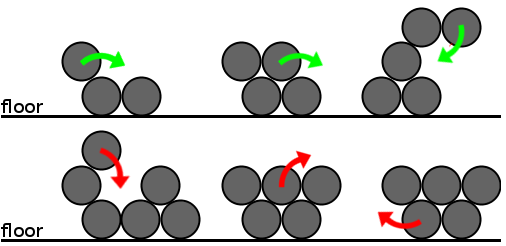
\includegraphics[width=.6\linewidth]{images/reconfiguration/constraints}
	\hfill
	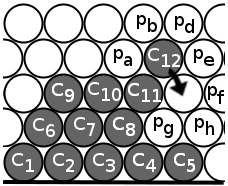
\includegraphics[width=.37\linewidth]{images/reconfiguration/named-system}
	\caption{On the left, motion constraints in our model: examples of feasible (at the top) and infeasible moves (at the bottom). On the right, a labeled system: gray cells are occupied by a module, whereas white cells are empty. Some of the empty cells are labeled with their position (e.g., $p_a$, $p_b$, etc.).}
	\label{fig:reconfiguration:motion-constraint}
	\label{fig:reconfiguration:named-system}
\end{figure}

$p_{C_i} = (x_{C_i},y_{C_i})$ denotes the coordinates of the 2D Catom $C_i$ in the horizontal hexagonal lattice. $p_{C_i}.x$ denotes the column of $C_i$ in the lattice, while $p_{C_i}.y$ denotes the row of $C_i$. For instance, in Figure~\ref{fig:reconfiguration:named-system}, $p_{C_2}.y = 0$ and $p_{C_9}.y = 2$. We assume that, at any time, modules know both their coordinates in the lattice and the coordinates of their neighbor through an external algorithm, e.g.,~\cite{funiak-ijrr08} or a distributed and incremental version of~\cite{moffo2016first}.

Moreover, a 2D Catom can roll \gls{cw} or \gls{ccw} around a stationary module. During an atomic move, a module rotates $60°$, going from one cell of the lattice to its adjacent cell. We assume that a 2D Catom has only the capability to lift itself, it cannot carry or push other modules. A module can move if it satisfies the freedom of movement rule (see Rule~\ref{rule:freedom-movement}).

\begin{myRule}[the freedom of movement rule]
	\label{rule:freedom-movement}
	Because of possible mismatching issues due to physical constraints, a 2D Catom can only move from/into a cell if this cell is currently unoccupied and if no two symmetrically opposing cells adjacent to that cell are occupied (see Figure~\ref{fig:reconfiguration:motion-constraint}). Furthermore, we consider the floor as if it were filled with 2D Catoms. If a 2D Catom, $C_i$, satisfies the freedom of movement rule, $free(C_i)$ is true, otherwise it is false.
\end{myRule}

We assume that 2D Catoms are not provided with any hardware mechanism to handle collision. Thus, collisions have to be prevented by the self-reconfiguration algorithm, using communications. 

We use $\mathcal{N}^{K}_{p}$ to denote the set of modules geographically adjacent to position $p$.  A module ${C_i}$, moving from $p_{C_i}$ to $p^{\prime}_{C_i}$, is somewhere between these two positions, and thus, ${C_i}$ belongs to the set of geographically adjacent modules of all the cells adjacent to $p_{C_i}$ or $p^{\prime}_{C_i}$. For instance, in the labeled system depicted in Figure~\ref{fig:reconfiguration:named-system}, module $C_{12}$ is moving and thus it belongs to $\mathcal{N}^{K}_{p_a}$, $\mathcal{N}^{K}_{p_b}$, $\mathcal{N}^{K}_{p_d}$, $\mathcal{N}^{K}_{p_{C_{12}}}$, $\mathcal{N}^{K}_{p_e}$, $\mathcal{N}^{K}_{p_{C_{11}}}$, $\mathcal{N}^{K}_{p^{\prime}_{C_{12}}}$, $\mathcal{N}^{K}_{p_f}$, $\mathcal{N}^{K}_{p_g}$ and $\mathcal{N}^{K}_{p_h}$. Note that in the presence of moving modules, $\mathcal{N}^{K}_{p_{C_{i}}}$ may be different from $\mathcal{N}^{N}_{C_{i}}$. Also notice that the construction of the $\mathcal{N}^{K}$ sets is not automatic. 2D Catoms are not equipped with any presence sensor. Maintaining on Catoms the $\mathcal{N}^{K}$ set of some specific nearby positions, using only communications, is one of the key operations in the implementation of our distributed algorithm.

$\mathcal{I}$ and $\mathcal{G}$ denote the initial and the goal shapes, respectively. Our algorithm assumes some admissibility conditions for $\mathcal{I}$ and $\mathcal{G}$ (see Section~\ref{section:reconfiguration:at-a-glance}). We also consider that every module stores a representation of the shape geometry of $\mathcal{G}$. The goal shape can be stored efficiently using Constructive Solid Geometry for Programmable Matter (CSG4PM)~\cite{tucci2017efficient}. CSG4PM encodes a vectorial representation of a shape using operations on primitive shapes. The shape can be scaled up without increasing the memory usage to store it. Moreover, CSG4PM provides processing-efficient methods of checking whether a given lattice cell belongs to the described shape or not. For instance, CSG4PM requires only 233 bytes to store goal configurations (shape and colors) similar to the car configurations in Figures~\ref{fig:reconfiguration:example-car} and \ref{fig:reconfiguration:shapes}, which are respectively composed of 120 and 9,644 modules.

Note that colors are used for illustration purposes only. The current prototype is not equipped with any mechanism to glow with color. It is possible to do so, but the weight of that color mechanism will probably change the 2D Catom motion speed (see Section~\ref{section:context:catom2D}).

Furthermore, we assume a failure-free environment, i.e., we assume there is no module, communication, move or lattice failure during the algorithm execution.

\section{State of the Art}
\label{section:reconfiguration:related-work}

Self-reconfiguration and self-assembly have attracted a lot of attention in the last two decades. Algorithms have been proposed for modules of different shapes, with different physical motion constraints and arranged in various ways. In this chapter, we only consider the self-reconfiguration of systems composed of elements organized in a vertical and two-dimensional hexagonal lattice. Algorithms also differ by their restrictions on the initial and goal shapes. Our algorithm can manage almost any kind of initial and goal compact shapes (see Section~\ref{section:reconfiguration:at-a-glance}). Algorithms also vary in their control properties. In particular, they can be centralized or distributed, and synchronous or asynchronous.

In~\cite{walter2000distributed}, the authors propose a distributed algorithm to perform chain-to-chain self-reconfiguration in a hexagonal lattice. Modules move in synchronous rounds. This work was later extended in order to allow self-reconfiguration from a chain configuration into an arbitrary shape with some admissibility conditions~\cite{walter2005algorithms,bateau2012increasing}. These algorithms assume less restrictive motion constraints than those we assume for the 2D Catoms. For instance, these algorithms allow the first two motions described as infeasible in Figure~\ref{fig:reconfiguration:motion-constraint}, starting from the left.

In~\cite{hurtado2013distributed}, Hurtado et al. propose a self-reconfiguration algorithm for modular robots arranged in a two-dimensional square or a two-dimensional hexagonal lattice. This algorithm is intended to run in a synchronized framework. The proposed method runs in two stages. It first reconfigures the robot from the initial configuration into a strip configuration and then from the strip configuration into the goal shape. A leader assigns a final destination location for every module in the strip configuration using a tree-based approach.

Self-reconfiguration presented in~\cite{lakhlef2014optimization,lakhlef2015energy,lakhlef2015fast} consists in using map-less representation for describing shapes. The benefit lies in a reduced memory footprint, but the number of supported goal shapes is limited. Proposed distributed algorithms manage to construct square shapes with spherical modules arranged in a two-dimensional hexagonal lattice. In \cite{lakhlef2015energy,lakhlef2015fast}, the authors propose to self-reconfigure a chain of modules into a square shape and demonstrate that the number of movements can be predicted. A more general algorithm designed to self-reconfigure arbitrary connected shapes into a square shape is presented in~\cite{lakhlef2014optimization}.

Algorithms allowing the reconfiguration of an initial clump of modules arranged in a hexagonal lattice into a chain configuration were proposed in~\cite{wong2013deterministic, wong2015unpacking}. These algorithms do not require message passing and do not use any pre-processing. In these algorithms, modules can both rotate and slide over other modules. Thus, these algorithms assume less restrictive motion constraints than ours.

In~\cite{de2006scalable}, the authors propose a distributed shape formation algorithm based on hole motions, for ensembles arranged in a hexagonal lattice. This algorithm can construct various shapes by randomly moving empty spaces within the ensemble. Although a wide variety of shapes can be built, this algorithm requires less restrictive motion constraints than ours, e.g., it allows the first two infeasible motions in Figure~\ref{fig:reconfiguration:motion-constraint}.

In~\cite{rubenstein2014programmable}, the authors propose a parallel, decentralized and asynchronous algorithm for the Kilobot swarm system~\cite{rubenstein2014programmable} to self-assemble almost any kind of compact two-dimensional shapes. This algorithm has been applied to hardware systems with more than a thousand individual robots per swarm entity. However, these swarm robots have different physical motion constraints. During the self-assembly process, Kilobots may collide with one another. While this is possible with Kilobots, this is not acceptable in our system.

Table~\ref{table:reconfiguration:state-art} summarizes the related work. Existing algorithms contain interesting ideas but consider different physical motion constraints, different restrictions on the initial and goal shapes and different control properties. The contribution of this chapter is to propose a distributed, fully decentralized, asynchronous and parallel self-reconfiguration algorithm for 2D Catoms that can manage almost any kind of initial and final compact shapes.

{
			\newcommand{\lenMinusOne}{0.08\linewidth}
			\newcommand{\lenZero}{0.09\linewidth}
			\newcommand{\lenOne}{0.12\linewidth}
			\newcommand{\lenTwo}{0.14\linewidth}
			\newcommand{\lenThree}{0.18\linewidth}
			\newcommand{\lenFour}{0.22\linewidth}
			\newcommand{\lenFive}{0.27\linewidth}
			\newcommand{\lenSix}{0.28\linewidth}
			
			\begin{table}[!h]
				\small
				\begin{center}
					\begin{tabular}{|C{\lenFive}|C{\lenThree}|C{\lenTwo}|C{\lenSix}|}
						\hline
						Cite & Shapes & Module movement capabilities & Collision and deadlock avoidance \\
						\hline
						\cite{walter2000distributed} & chain to chain & relaxed & centralized pre-computation, synchronous rounds\\
						\hline
						\cite{walter2005algorithms,bateau2012increasing} & chain to 2D & relaxed & centralized pre-computation, synchronous rounds\\
						\hline
						\cite{hurtado2013distributed} & 2D & UN & synchronized framework, single direction, intermediate configuration and priority numbers\\
						\hline 
						\cite{lakhlef2015energy, lakhlef2015fast} & chain to square & relaxed and very relaxed & predefined shape construction\\
						\hline
						\cite{lakhlef2014optimization} & arbitrary connected to square & relaxed & predefined shape construction\\
						\hline
						\cite{wong2015unpacking} & compact 2D to chain & relaxed & touch sensors, synchronous rounds, single direction\\
						\hline
						\cite{de2006scalable} & 2D & relaxed & UN \\
						\hline
						\cite{rubenstein2014programmable} & horizontal 2D compact & very relaxed & collision allowed (swarm robotic) \\
						\hline
					\end{tabular}
				\end{center}
			
				\begin{center}
					\begin{tabular}{|C{\lenFive}|C{\lenThree}|C{\lenTwo}|C{\lenSix}|}
						\hline
						Our Contribution: C2SR  & vertical 2D compact & strict & messages, single direction\\
						\hline
					\end{tabular}
				\end{center}
			\caption{Summary of the state of the art on self-reconfiguration in MSRs where modules are arranged in a hexagonal lattice. ``UN'' stands for ``Unknown''.\label{table:reconfiguration:state-art}}
			\end{table}
}

\section{C2SR Algorithm at a Glance}
\label{section:reconfiguration:at-a-glance}

In this section, we present the general idea of the Cylindrical-Catoms Self-Reconfiguration (C2SR) algorithm that reconfigures a robot composed of modules from an initial shape $\mathcal{I}$ into a goal one $\mathcal{G}$. 

Both shapes have to satisfy some admissibility conditions. We provide some intuitions about them in this paragraph and in Figure~\ref{fig:reconfiguration:admissibility}. A more formal description of the conditions and their demonstration are left for future work. Both shapes are compact, i.e., they do not contain holes, they are homeomorphic to a sphere. Moreover, both shapes are next to each other and intersect in one or more bottom cells. Let the peripheral path be the path formed from the empty cells on the periphery of both shapes, starting from and ending at the second horizontal layer (see Figure~\ref{fig:reconfiguration:admissibility}). This path has to be large enough to allow some modules, which progress along that path in the same direction with an empty space of at least one cell between successive modules, to move without violating our motion constraints and without risking colliding/getting attached to one another (see Figure~\ref{fig:reconfiguration:admissibility} and Rule~\ref{rule:freedom-movement}). Note that this condition implies that, in the upper layers, the horizontal space between the initial shape and the goal shape has to be sufficiently large to enable these modules to move between the two shapes. Furthermore, the number of 2D Catoms in $\mathcal{I}$ has to be greater than or at least equal to the number of target positions in $\mathcal{G}$ (i.e., $|\mathcal{I}| \geq |\mathcal{G}|$).

\begin{figure}[!h]
	\centering
	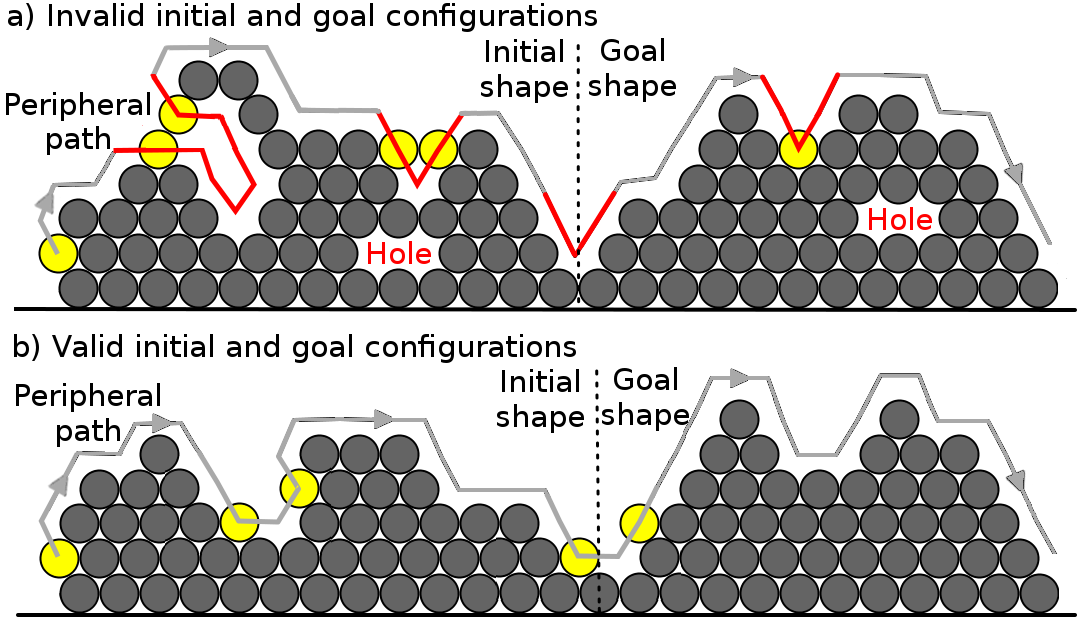
\includegraphics[width=0.7\linewidth]{images/reconfiguration/admissibility}
	\caption{Invalid (at the top) and valid (at the bottom) initial and goal configurations in C2SR. Modules in yellow, which are not part of the initial or goal shapes, progress along the peripheral path in the same direction with an empty space of at least one cell between successive modules. The configurations at the top are not valid for several reasons. First, they do not intersect in at least one cell. Second, they both contain a hole. Third, the peripheral path is not large enough at the locations in red. Indeed, the modules in yellow could not move without violating our motion constraints and without getting attached to each other.}
	\label{fig:reconfiguration:admissibility}
\end{figure}

During the execution of C2SR with shapes individually composed of only continuous horizontal layers, the goal shape is progressively constructed from the bottom layer to the top one by stripping the initial shape, module by module in reverse order (see Figure~\ref{fig:reconfiguration:car-construction-process}). Because of physical constraints, at a given instant, only modules on the periphery can move. In order to avoid module collisions and deadlocks, peripheral modules form a stream: modules roll in the same direction $d$ (CW in Figures~\ref{fig:reconfiguration:example-car} and~\ref{fig:reconfiguration:car-construction-process}), and maintain an empty cell between one another using message exchanges. Modules in the stream do not overtake one another.

\begin{figure}[!h]
	\centering
	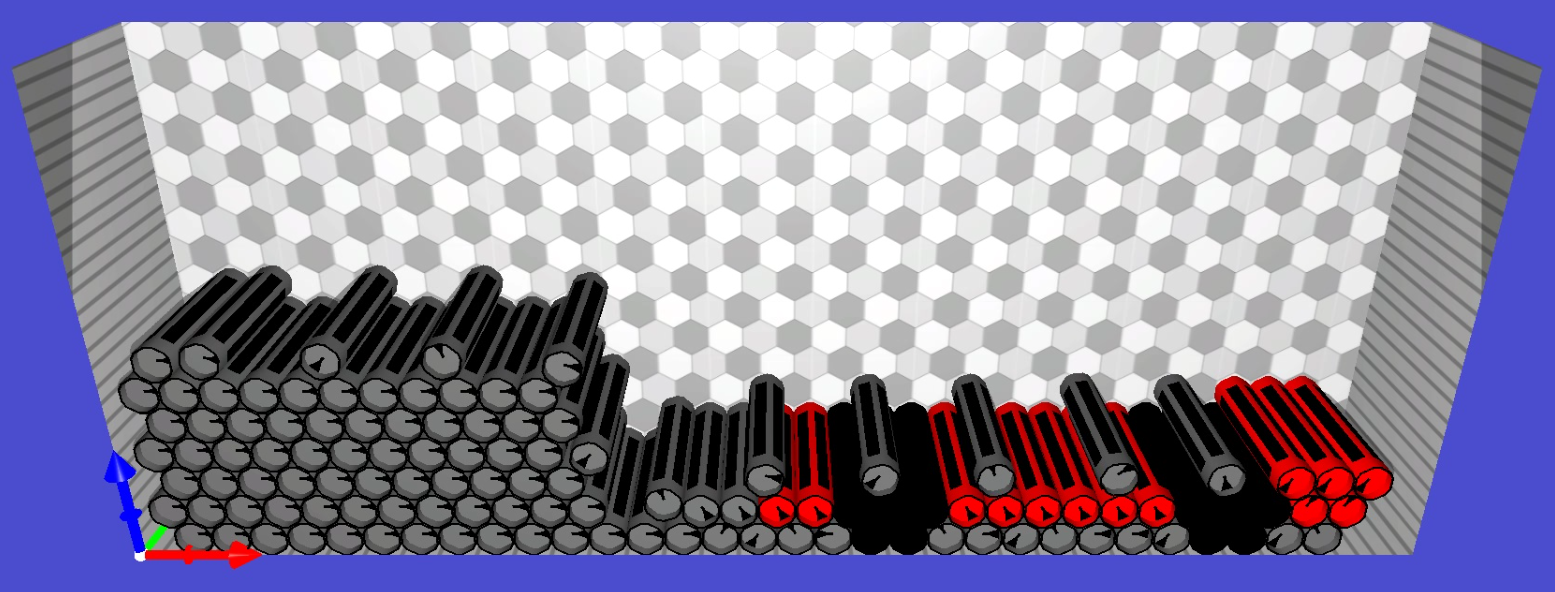
\includegraphics[width=0.7\textwidth]{images/reconfiguration/car-construction-process}
	\caption{Screenshot during the self-reconfiguration process using C2SR with the initial and goal shapes of Figure~\ref{fig:reconfiguration:example-car}. The modules in the stream progress by rotating CW.}
	\label{fig:reconfiguration:car-construction-process}
\end{figure}

C2SR is based on a set of states and transition rules. Figure~\ref{fig:reconfiguration:c2sr-state-diagram} shows the state diagram of our algorithm. Modules can have different states, namely INIT, BLOCKED, WAITING, MOVING, or GOAL. Modules are initially in the INIT state. Modules in the WAITING and MOVING states belong to the stream. Figure~\ref{fig:reconfiguration:c2sr-state-example} shows the different states of the modules in Figure~\ref{fig:reconfiguration:car-construction-process}.

\begin{figure}[!h]
	\centering
	\begin{tikzpicture}[>=stealth',shorten >=1pt,auto,node distance=4.5cm,line width=0.025cm]
%line width=0.025cm

   \tikzstyle{every state}=[minimum size=1.75cm]
  \node[initial,state] (init)      {INIT};
  \node[state,accepting] (conv) [below of=init]  {GOAL};
  \node[state]  (bloc) [right of=init] {BLOCKED};
  \node[state]  (wait) [below of=bloc] {WAITING};
  \node[state]  (mov) [right of=wait] {MOVING};

%, line width=0.1cm
 \path [->] (init) edge  node {$\neg stream$} (bloc)
            edge [left] node {$converged$} (conv)
			edge node {$stream$} (wait)
		(bloc) edge node {$stream$} (wait)
	     (wait) edge [below] node {$progression$} (mov)
		(mov) edge [bend right,above] node  {$\neg converged$} (wait)
		(mov) edge [bend left] node  {$converged$} (conv);
		
\end{tikzpicture}
	\caption{C2SR state diagram.\label{fig:reconfiguration:c2sr-state-diagram}}
\end{figure}

A module locally decides to start taking part in the stream if it satisfies the stream entrance rule (see Rule~\ref{rule:stream-entrance}). Intuitively, a free module enters the stream if moving in the direction $d$ consists in: moving around a module on the ground or descending $\mathcal{I}$.

\begin{myRule}[the stream entrance rule]
	\label{rule:stream-entrance}
	Let us consider two modules $C_i$ and $C_j$ such that both $C_i$ and $C_j$ are on the periphery and $C_j$ is the next peripheral neighbor of $C_i$ in the direction of rotation, $d$. $p^{\prime}_{C_i}$ denotes the position that $C_i$ would occupy after its rotation around $C_j$. $C_i$ decides to take part in the stream if the following logical condition is satisfied:
	\begin{align*}
		% \neg converged(C_i)
		stream(C_i) :-\ & state(C_i) \neq \text{GOAL} \ \text{\footnotesize // has not converged yet}\\
		\land\ \ \ & free(C_i)\ \text{\footnotesize // mechanical constraints}\\
		\land\ (\ & (p_{C_i} \notin \mathcal{G} \land p_{C_j}.y = 0)\ \text{\footnotesize // move around a module on the ground} \\
		\lor\ & (p_{C_i} \notin \mathcal{G} \land p^{\prime}_{C_i}.y \leq p_{C_i}.y)\ )\ \text{\footnotesize // descend $\mathcal{I}$}\\
	\end{align*}
\end{myRule}

\begin{figure}
	\centering
	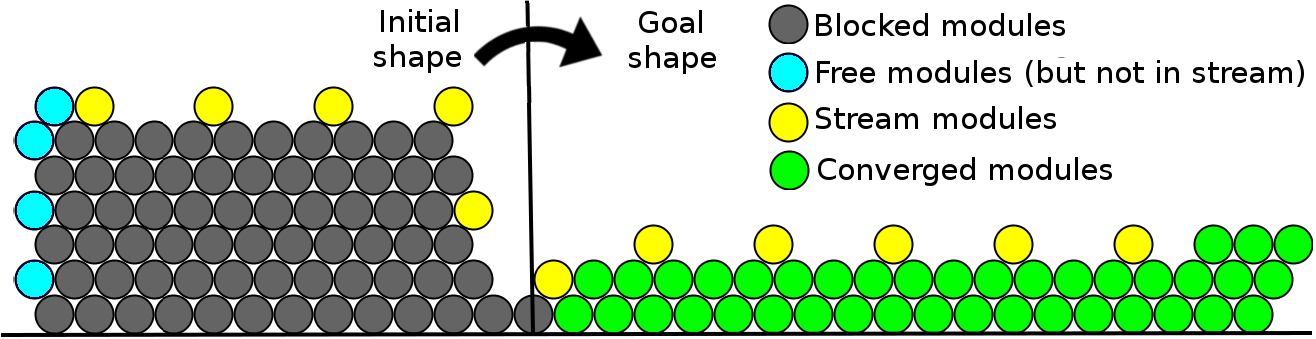
\includegraphics[width=0.7\linewidth]{images/reconfiguration/stream-entrance}
	\caption{Different module states in C2SR. Note that, at this particular moment of the reconfiguration, no Catom is in the moving state.}
	\label{fig:reconfiguration:c2sr-state-example}
\end{figure}

A module in the stream decides to move if it satisfies the stream progression rule (see Rule~\ref{rule:stream-progression}). More precisely, a module in the stream can move if the set of modules geographically adjacent to its destination cell contains no more than three modules and none of them, except the module itself, belongs to the stream (see Figure~\ref{fig:reconfiguration:progression}). This rule requires local interactions with neighbors adjacent to its source and destination positions. These modules are at most two cells away. The admissibility conditions on $\mathcal{I}$, combined with the two rules above, guarantee that these modules are five network hops away at most.

\begin{myRule}[the stream progression rule]
	\label{rule:stream-progression}
	A module $C_i$ can move from its position $p_{C_i}$ to the position $p^{\prime}_{C_i}$ if the following condition is satisfied:
	\begin{align*}
	progression(C_i) :-\ & state(C_i) = \text{WAITING}\ \text{\footnotesize // in the stream}\\
	& \land |\mathcal{N}^{K}_{p^{\prime}_{C_i}}| \leq 3 \ \text{\footnotesize // no more than 3 modules near the destination cell}\\
	& \text{~~~~~~~~~~~~~\footnotesize // no other stream module in the surroundings of the destination cell:}\\
	& \land \nexists C_j \in \mathcal{N}^{K}_{p^{\prime}_{C_i}}\mid  C_j \neq C_i \land (state(C_i) = \text{WAITING} \lor state(C_i) = \text{MOVING})
	\end{align*}
\end{myRule}

\begin{figure}[!h]
	\centering
	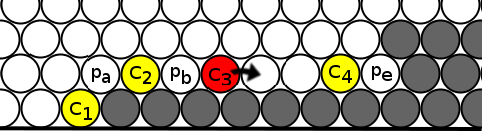
\includegraphics[width=0.7\linewidth]{images/reconfiguration/progression}
	\caption{C2SR stream progression rule: a simple example. Modules should rotate CW. White cells are empty and some of them are labeled with their position in the lattice (e.g., $p_a$, $p_b$, etc.). Modules $C_1$, $C_2$, $C_3$ and $C_4$ are in the stream. $C_3$ is moving. $C_1$ cannot move because $C_2$ is in the stream and $C_2 \in \mathcal{N}^{K}_{p_a}$. $C_2$ cannot move because $C_3$ is in the stream and $C_3 \in \mathcal{N}^{K}_{p_b}$. $C_3$ can move to $p^{\prime}_{C_3}$ because $\mathcal{N}^{K}_{p^{\prime}_{C_3}}$ contains only three modules and none of them is in the stream, except for $C_3$. $C_4$ cannot move because $|\mathcal{N}^{K}_{p_e}| = 5$.}
	\label{fig:reconfiguration:progression}
\end{figure}

Rule~\ref{rule:stream-progression} prevents collisions. The admissibility conditions on $\mathcal{I}$ and $\mathcal{G}$, combined with Rules~\ref{rule:stream-entrance}~and~\ref{rule:stream-progression}, prevent deadlock. Note that, because of the stripping order and the construction order, our algorithm also guarantees that, at all times the system remains connected.

Each module checks for convergence using Rule~\ref{rule:local-convergence} at initialization and after every move. A module has converged if it is initially in a goal position, or if it has reached $\mathcal{G}$ and moving in the direction $d$ will cause it to leave $\mathcal{G}$ or to go up.

\begin{myRule}[the local convergence rule]
	\label{rule:local-convergence}
	Let us consider two modules $C_i$ and $C_j$ such that both $C_i$ and $C_j$ are on the periphery and $C_j$ is the next peripheral neighbor of $C_i$ in the direction of rotation. $p^{\prime}_{C_i}$ denotes the position that $C_i$ would occupy after its rotation around $C_j$. $C_i$ has converged if it satisfies the following condition:
	\begin{align*}
converged(C_i) :-\ & (state(C_i) = \text{INIT} \land p_{C_i} \in \mathcal{G})\ \text{\footnotesize // initially in $\mathcal{G}$}\\
& \lor (p_{C_i} \in \mathcal{G} \land p^{\prime}_{C_i} \notin \mathcal{G})\ \text{\footnotesize // about to leave $\mathcal{G}$} \\
& \lor (p_{C_i} \in \mathcal{G} \land p^{\prime}_{C_i} \in \mathcal{G} \land p^{\prime}_{C_i}.y > p_{C_i}.y)\ \text{\footnotesize // about to go up in $\mathcal{G}$}
	\end{align*}
\end{myRule}

Applying these rules in a distributed asynchronous system with parallel communications and motions is challenging. It is especially complex to maintain $\mathcal{N}^K$ sets using only communications. A complete implementation that overcomes this challenge is presented in the next section.

\section{C2SR Implementation}
\label{section:reconfiguration:algorithm}

In this section, we provide a detailed implementation of C2SR\footnote{The complete source code of C2SR is available online at: \VisibleSimUrl{}}. Algorithm \ref{alg:reconfiguration:c2sr:init} shows the input and local variables of C2SR along with its initialization pseudo-code. Every module knows its position in the lattice, the goal shape, $\mathcal{G}$, and the rotation direction, $d$. Algorithm \ref{alg:reconfiguration:c2sr:helpers} describes some helper functions used in the description of our implementation of C2SR. Algorithm \ref{alg:reconfiguration:c2sr:msg} provides the message handler pseudo-code of C2SR. Algorithm \ref{alg:reconfiguration:c2sr:move} gives the pseudo-code executed by a module after it has finished an atomic move. We assume that interrupts are disabled during message and event handler execution. 

{
\myAlg{	
		\Input{}
		\nonl $p_{C_i}$ \tcp{\footnotesize position of  $C_i$}
		\nonl $d \in \{CW, CCW\}$ \tcp{\footnotesize direction of rotation}
		\nonl $\mathcal{G}$ \tcp{\footnotesize goal shape}

		
		\Variables{}
		\nonl $state$ \tcp{\footnotesize state of  $C_i$}
		\nonl $Movings$ \tcp{\footnotesize cells from/into which a neighbor module is moving}
		\nonl $Pendings$ \tcp{\footnotesize pending clearance requests}
		\nonl $clearance$ \tcp{\footnotesize clearance for the current move (if any)}
		
		\BlankLine
		\BlankLine
		
		{\bf Initialization} of $C_i$:\\
		
		$Movings \gets \emptyset$; 	$Pendings \gets \emptyset$; $clearance \gets \perp$\;
		\uIf {$p_{C_i} \in \mathcal{G}$} {
			$state \gets \mathrm{GOAL}$\; \label{alg:reconfiguration:c2sr:line:state-1}
		} \uElseIf{$isInStream()$} {
			$state \gets \mathrm{WAITING}$\; \label{alg:reconfiguration:c2sr:line:state-2}
			$requestClearance()$\;
		} \Else {
			$state \gets \mathrm{BLOCKED}$\;
		}
		\caption{C2SR algorithm input, local variables and initialization detailed for any module ${C_i}$.\label{alg:reconfiguration:c2sr:init}\vspace{3em}}
}

\myAlgTwoPages{
		\Fn{hasConverged()}{
			\tcp{The local convergence rule (Rule \ref{rule:local-convergence})}
			\Return converged($C_i$)\;
		}
		
		\BlankLine	
		\BlankLine
		
		\Fn{areAdjacentCells($p_1,p_2$)}{
			\Return true if cells at positions $p_1$ and $p_2$ are adjacent in the hexagonal lattice, false otherwise\;
		}
		
		\BlankLine
		\BlankLine
		
		\Fn{oppositeDirection($d$)} {
			\tcp{$d \in \{CW, CCW\}$}
			\Return the opposite direction of $d$\;
		}
		
		\BlankLine
		\BlankLine
		
		\Fn{isFree()}{
			\tcp{The freedom of movement rule (Rule \ref{rule:freedom-movement})} 
			\Return free($C_i$) considering both $\mathcal{N}^{N}_{C_i}$ and $Movings$\;
		}
		
		\BlankLine
		\BlankLine
		
		\Fn{isInStream()}{
			\tcp{The stream entrance rule (Rule \ref{rule:stream-entrance})}
			\Return stream($C_i$) considering both $\mathcal{N}^{N}_{C_i}$ and $Movings$\;
		}
		
		\BlankLine
		\BlankLine
		
		\Fn{getNeighbor($dir$)}{
			%\tcp{Require empty neighbor cells to be consecutive around $C_i$}
			\Return the peripheral neighbor in direction $dir$ (see Section \ref{section:reconfiguration:model})\;
		}
		
		\BlankLine
		\BlankLine
		
		\Fn{getNeighbor($dir,pos$)}{
			\Return $C_k \in \mathcal{N}^{N}_{C_i}$ such that $C_i$ is connected to $C_k$ on the connected interface that immediately follows the interface pointing to position $pos$ in direction $dir$\;
		}			
}{
		\setcounter{AlgoLine}{14}

		\Fn{requestClearance()}{
			$C_k \gets getNeighbor(d)$\;
			$p^{\prime}_{C_i} \gets$ position after rotation in direction $d$ around $C_k$\;
			$r \gets (src \gets p_{C_i}, dest \gets p^{\prime}_{C_i}, cnt \gets 0)$\;		
			{\bf send} CLEARANCE\_REQUEST($r$) {\bf to} $C_k$\;
		}
		\BlankLine	
		\BlankLine
		
		\Fn{forwardClearance($c(src,dest), C_j$)}{
			\uIf{areAdjacentCells($c.src,p_{C_i}$)}{
				$C_k \gets getNeighbor(oppositeDirection(d),c.src)$\;
				\uIf{$C_k \ne C_j$ AND $areAdjacentCells(c.src,p_{C_k})$}{
					{\bf send} CLEARANCE(c) {\bf to} $C_k$\;
				} \Else {
					$Movings \gets Movings \cup \{c.src\}$\;
					{\bf send} CLEARANCE(c) {\bf to} $C_l \mid p_{C_l} = c.src$\;
				}
			}\ElseIf{areAdjacentCells($c.dest,p_{C_i}$)}{
				$C_k \gets getNeighbor(oppositeDirection(d),c.dest)$\;
				{\bf send} CLEARANCE($c$) {\bf to} $C_k$\;
			}
		}
		
		\BlankLine	
		\BlankLine
		
		\Fn{forwardEndOfMove($c(src,dest), C_j$)}{
			\uIf{areAdjacentCells($c.src,p_{C_i}$)} {
				$C_k \gets getNeighbor(oppositeDirection(d),c.src)$\;
				\If{$C_k \ne C_j$ AND $areAdjacentCells(c.src,p_{C_k})$}{
					{\bf send} END\_OF\_MOVE($c$) {\bf to} $C_k$\;	
				}
			} \ElseIf {areAdjacentCells($c.dest,p_{C_i}$)} {
				$C_k \gets getNeighbor(oppositeDirection(d),c.dest)$\;
				{\bf send} END\_OF\_MOVE($c$) {\bf to} $C_k$\;
			}
		}
		\caption{C2SR helper functions detailed for any module ${C_i}$.\label{alg:reconfiguration:c2sr:helpers}}
}

\myAlgTwoPages{
		{\bf When} CLEARANCE\_REQUEST($r(src,dest,cnt)$) {\bf is received by} ${C_i}$
		{\bf from} ${C_j}$ {\bf do}:
		
		\label{alg:reconfiguration:c2sr:line:check-clearance-start}		
		\If {$state = \mathrm{WAITING}$} {				
			\label{alg:reconfiguration:c2sr:line:delayed-clearance-out1-start}
			{\bf send} DELAYED\_CLEARANCE($r$) {\bf to} $C_j$\;
			\Return\;
		} 
		\label{alg:reconfiguration:c2sr:line:delayed-clearance-out1-end}
		
		\If{$r.dest \in Movings$} {
			\label{alg:reconfiguration:c2sr:line:delayed-clearance-in-start}	
			$Pendings \gets Pendings \cup \{r\}$\; 	
			\Return\;				
		} 
		\label{alg:reconfiguration:c2sr:line:delayed-clearance-in-end}	
		
		\If {$state = \mathrm{BLOCKED}$ OR $state = \mathrm{GOAL}$} {
			
			\If {r.cnt = 3} {
				\label{alg:reconfiguration:c2sr:line:delayed-clearance-out2-start}
				{\bf send} DELAYED\_REQUEST($r$) {\bf to} $C_j$\;
				\Return\;
			}
			\label{alg:reconfiguration:c2sr:line:delayed-clearance-out2-end}
			
			$r.cnt \gets r.cnt + 1$\;
		}
		
		$C_n \gets getNeighbor(d,r.dest)$\;
		
		\uIf {$C_n \neq C_j$ AND $areAdjacentCells(p_{C_n},r.dest)$} {
			{\bf send} CLEARANCE\_REQUEST($r$) {\bf to} $C_n$\;
		} \Else {
			\label{alg:reconfiguration:c2sr:line:clearance-granted-1-start}
			$c \gets (r.src,r.dest)$\;
			$Movings \gets Movings \cup \{r.dest\}$\;
			$forwardClearance(c, \perp)$\;
		}
		\label{alg:reconfiguration:c2sr:line:clearance-granted-1-end}
		\label{alg:reconfiguration:c2sr:line:check-clearance-end}
		
		\BlankLine
		\BlankLine
		

}{

		\setcounter{AlgoLine}{19}
		{\bf When} CLEARANCE($c(src,dest)$) {\bf is received by} ${C_i}$
		{\bf from} ${C_j}$ {\bf do}:
		
		\label{alg:reconfiguration:c2sr:line:clearance-forward-start}	
		\uIf{$c.src = p_{C_i}$} {
			$clearance \gets c$\;
			{\bf send} START\_TO\_MOVE {\bf to} $C_j$\;
		} \Else {
			$forwardClearance(c, C_j)$\;
		}
		\label{alg:reconfiguration:c2sr:line:clearance-forward-end}	
		
		\BlankLine
		\BlankLine
		
		{\bf When} DELAYED\_CLEARANCE($r(src,dest,cnt)$) {\bf is received by} ${C_i}$
		{\bf from} ${C_j}$ {\bf do}:
		
		\label{alg:reconfiguration:c2sr:line:delayed-clearance-msg-start}
		\If {$r.src \ne p_{C_i}$}{
			$Pendings \gets Pendings \cup \{r\}$\;
		}
		\label{alg:reconfiguration:c2sr:line:delayed-clearance-msg-end}	
		
		\BlankLine
		\BlankLine
		
		{\bf When} START\_TO\_MOVE {\bf is received by} ${C_i}$
		{\bf from} ${C_j}$ {\bf do}:
		\label{alg:reconfiguration:c2sr:line:start-move-and-ack-start}
		
		{\bf send} START\_TO\_MOVE\_ACK {\bf to} $C_j$\;
		
		\BlankLine
		\BlankLine
		
		{\bf When} START\_TO\_MOVE\_ACK {\bf is received by} ${C_i}$
		{\bf from} ${C_j}$ {\bf do}:
		
		$state \gets \mathrm{MOVING}$\;
		$C_k \gets getNeighbor(d)$\;
		{\bf move around} $C_k$ {\bf in direction} $d$\;
		\label{alg:reconfiguration:c2sr:line:start-move-and-ack-end}
		\BlankLine
		\BlankLine

		{\bf When} END\_OF\_MOVE($c(src,dest)$) {\bf is received by} ${C_i}$
		{\bf from} ${C_j}$ {\bf do}:
		
		\label{alg:reconfiguration:c2sr:line:end-of-move-start}
		$Movings \gets Movings - \{c.src, c.dest\}$\;
		$forwardEndOfMove(c, C_j)$\;
		\uIf{$isInStream()$}{
			$state \gets \mathrm{WAITING}$\; \label{alg:reconfiguration:c2sr:line:state-3}
			$requestClearance()$\;
		} \ElseIf {$\exists r \in Pendings \mid r \in areAdjacentCells(r.dest,c.src)$} {
			\label{alg:reconfiguration:c2sr:line:reactivated-delayed-clearance-start}
			$C_n \gets getNeighbor(d,r.dest)$\;
			\uIf {$areAdjacentCells(r.dest,p_{C_n})$} {
				{\bf send} CLEARANCE\_REQUEST($r$) {\bf to} $C_n$\;
			} \Else {
				$cl \gets (r.src,r.dest)$\;
				$Movings \gets Movings \cup \{cl.dest\}$\;
				$forwardClearance(cl, \perp)$\;
			}
		}
		\label{alg:reconfiguration:c2sr:line:reactivated-delayed-clearance-end}
		\label{alg:reconfiguration:c2sr:line:end-of-move-end}	
		\caption{C2SR algorithm message handler detailed for any module ${C_i}$.\label{alg:reconfiguration:c2sr:msg}}
}

\myAlg{		
		{\bf When} ${C_i}$ {\bf has finished to move do}:
		
		$p_{C_i} \gets clearance.dest$\;
		{\bf send} END\_OF\_MOVE(clearance) {\bf to} $getNeighbor(d)$\;
		\label{alg:reconfiguration:c2sr:line:end-move-send}
		$clearance \gets \perp$\;
		\eIf {$hasConverged()$} {
				$state \gets \mathrm{GOAL}$\;
		} {
				$state \gets \mathrm{WAITING}$\; \label{alg:reconfiguration:c2sr:line:stream-entrance}
					$requestClearance()$\;
		}
				
		\caption{C2SR algorithm event handler detailed for any module ${C_i}$.\label{alg:reconfiguration:c2sr:move}}
}
}

At initialization and during the execution, modules locally decide their state using Rules~\ref{rule:freedom-movement},~\ref{rule:stream-entrance}~and~\ref{rule:local-convergence}. Modules in the stream move in the rotation direction $d$ around their peripheral neighbor in the $d$ direction. Before moving, modules have to ensure that the stream progression rule (Rule \ref{rule:stream-progression}) is satisfied. WAITING modules send CLEARANCE\_REQUEST messages to get the authorization to move. Clearance requests are composed of the module source position and of its destination. These requests travel around the module destination cell. At each hop, modules check if the requested move satisfies the stream progression rule (see Algorithm~\ref{alg:reconfiguration:c2sr:msg}, lines \ref{alg:reconfiguration:c2sr:line:check-clearance-start}-\ref{alg:reconfiguration:c2sr:line:check-clearance-end}). If the stream progression rule is not satisfied, the clearance request has either to be stored locally (see Algorithm~\ref{alg:reconfiguration:c2sr:msg}, lines \ref{alg:reconfiguration:c2sr:line:delayed-clearance-in-start}-\ref{alg:reconfiguration:c2sr:line:delayed-clearance-in-end}) or to be stored at the previous module using a DELAYED\_CLEARANCE message (see Algorithm~\ref{alg:reconfiguration:c2sr:msg}, lines \ref{alg:reconfiguration:c2sr:line:delayed-clearance-out1-start}-\ref{alg:reconfiguration:c2sr:line:delayed-clearance-out1-end}, \ref{alg:reconfiguration:c2sr:line:delayed-clearance-out2-start}-\ref{alg:reconfiguration:c2sr:line:delayed-clearance-out2-end} and \ref{alg:reconfiguration:c2sr:line:delayed-clearance-msg-start}-\ref{alg:reconfiguration:c2sr:line:delayed-clearance-msg-end}). If the stream progression rule is satisfied, the clearance is granted (see Algorithm~\ref{alg:reconfiguration:c2sr:msg}, lines \ref{alg:reconfiguration:c2sr:line:clearance-granted-1-start}-\ref{alg:reconfiguration:c2sr:line:clearance-granted-1-end}). The clearance is then progressively forwarded back to the module that has initiated the request (see Algorithm~\ref{alg:reconfiguration:c2sr:msg},  lines \ref{alg:reconfiguration:c2sr:line:clearance-forward-start}-\ref{alg:reconfiguration:c2sr:line:clearance-forward-end}). 

To prevent collision, modules maintain a list of neighbor cells from/into which a module is moving. After having moved to a new position, modules send an END\_OF\_MOVE (EOM for short) message that is progressively forwarded around the cell of their previous position (see Algorithm~\ref{alg:reconfiguration:c2sr:move}, line \ref{alg:reconfiguration:c2sr:line:end-move-send} and Algorithm \ref{alg:reconfiguration:c2sr:msg}, lines \ref{alg:reconfiguration:c2sr:line:end-of-move-start}-\ref{alg:reconfiguration:c2sr:line:end-of-move-end}). Upon reception of an EOM message, delayed clearances are potentially re-activated (see Algorithm~\ref{alg:reconfiguration:c2sr:msg}, lines \ref{alg:reconfiguration:c2sr:line:reactivated-delayed-clearance-start}-\ref{alg:reconfiguration:c2sr:line:reactivated-delayed-clearance-end}).

START\_TO\_MOVE and START\_TO\_MOVE\_ACK messages guarantee that no message is lost when a module decides to actually move (see Algorithm~\ref{alg:reconfiguration:c2sr:msg}, lines 
\ref{alg:reconfiguration:c2sr:line:start-move-and-ack-start}-\ref{alg:reconfiguration:c2sr:line:start-move-and-ack-end}).

Modules never need to communicate with modules farther than two cells away in the lattice, which means that, due to our requirements, modules never need to send messages that have to travel more than five hops. Thus, our algorithm uses only local interactions between modules.

\section{Experimental Evaluation}
\label{section:reconfiguration:evaluation}

We implemented C2SR and evaluated it using VisibleSim, our simulator for modular robotic systems. This section presents our experimental results. Through our experiments, we show the effectiveness of C2SR and its efficiency in terms of communications, movements and execution time.

VisibleSim enables one to perform simulations with different and variable motion and communication delays. In our evaluation, we assume that neighboring modules communicate together using 8-N-1 serial communications. Hence, we assume that the effective bitrate is equal to 80\% of the link bitrate. We assume that the effective average communication bitrate between two neighboring modules follows a Gaussian distribution. Moreover, we assume that the average motion speed during the atomic moves of a 2D Catom also follows a Gaussian distribution. We do not simulate delays due to processing and interruptions as we assume them to be negligible in comparison to communication and motion delays.

Unless explicitly mentioned, we assume the following simulation parameters. We consider that the effective average communication bitrate during message exchanges between two neighboring modules has a distribution centered on 38.9~kbit/s with a standard deviation of 389~bit/s (1\% of the mean). In the current hardware prototype, a 2D Catom can move at a speed of 1.88~$mm \times s^{-1}$ (see Section~\ref{section:context:catom2D}). We assume that the average motion speed during the atomic moves of a module has a distribution centered on 1.88~$mm \times s^{-1}$ with a standard deviation of 0.0188~$mm \times s^{-1}$ (1\% of the mean).

We evaluate C2SR on the self-reconfiguration of random clumps of 2D Catoms into four kinds of shapes, namely a car, a flag, a magnet and a pyramid shape (see Figures~\ref{fig:reconfiguration:example-car} and~\ref{fig:reconfiguration:shapes}). For each target shape, we generated different versions of the goal configurations using different scales ranging from a dozen to ten thousand modules. For every single point on the result plots, 10 were performed.

\subsection{Effectiveness Evaluation}

As shown in Figure~\ref{fig:reconfiguration:shapes}, C2SR is able to self-reconfigure ensembles composed of more than 10,000 2D Catoms.

{
	\newcommand{\mySubfigureWidth}{120px}
	\newcommand{\mySubfigureHeight}{90px}
	\begin{figure}[h!]
		\centering			
		\small
		\begin{tabular}{c c}
			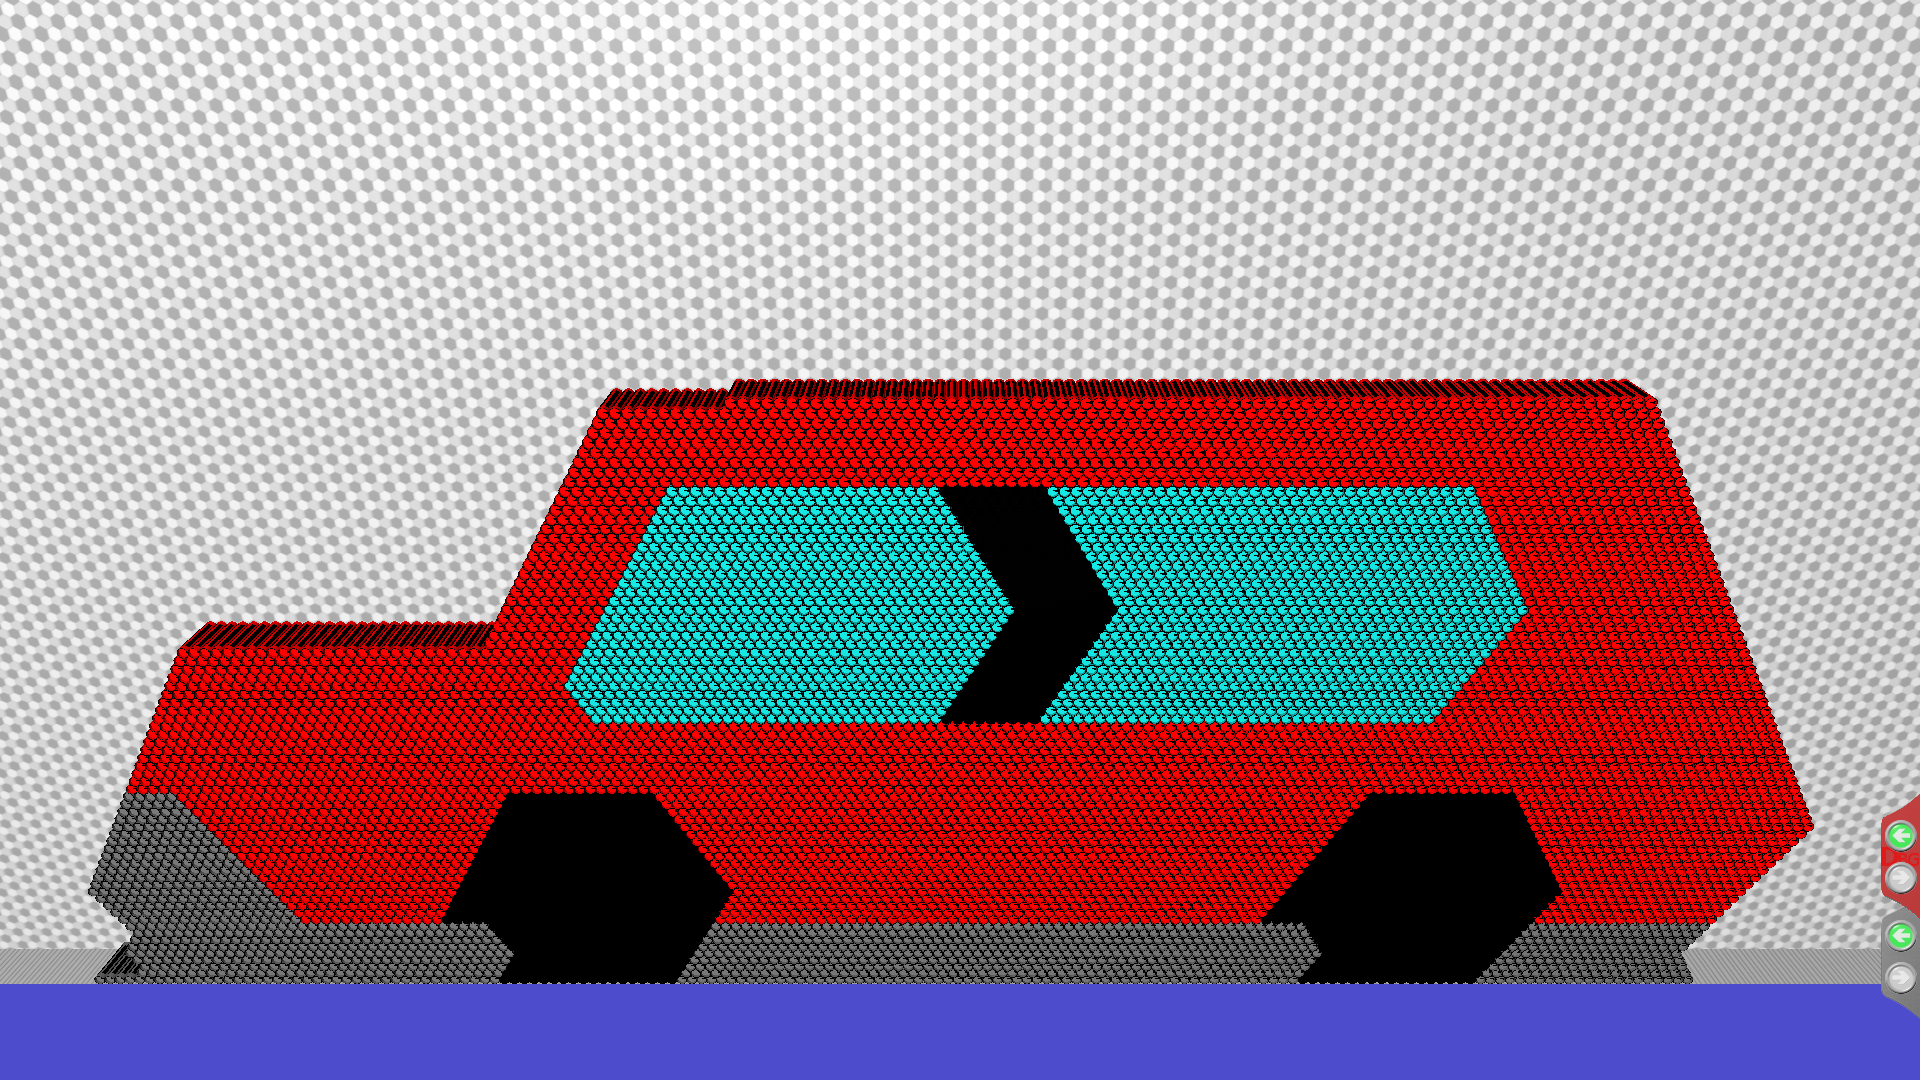
\includegraphics[width=\mySubfigureWidth,height=\mySubfigureHeight]{images/reconfiguration/car-9644.png} & 	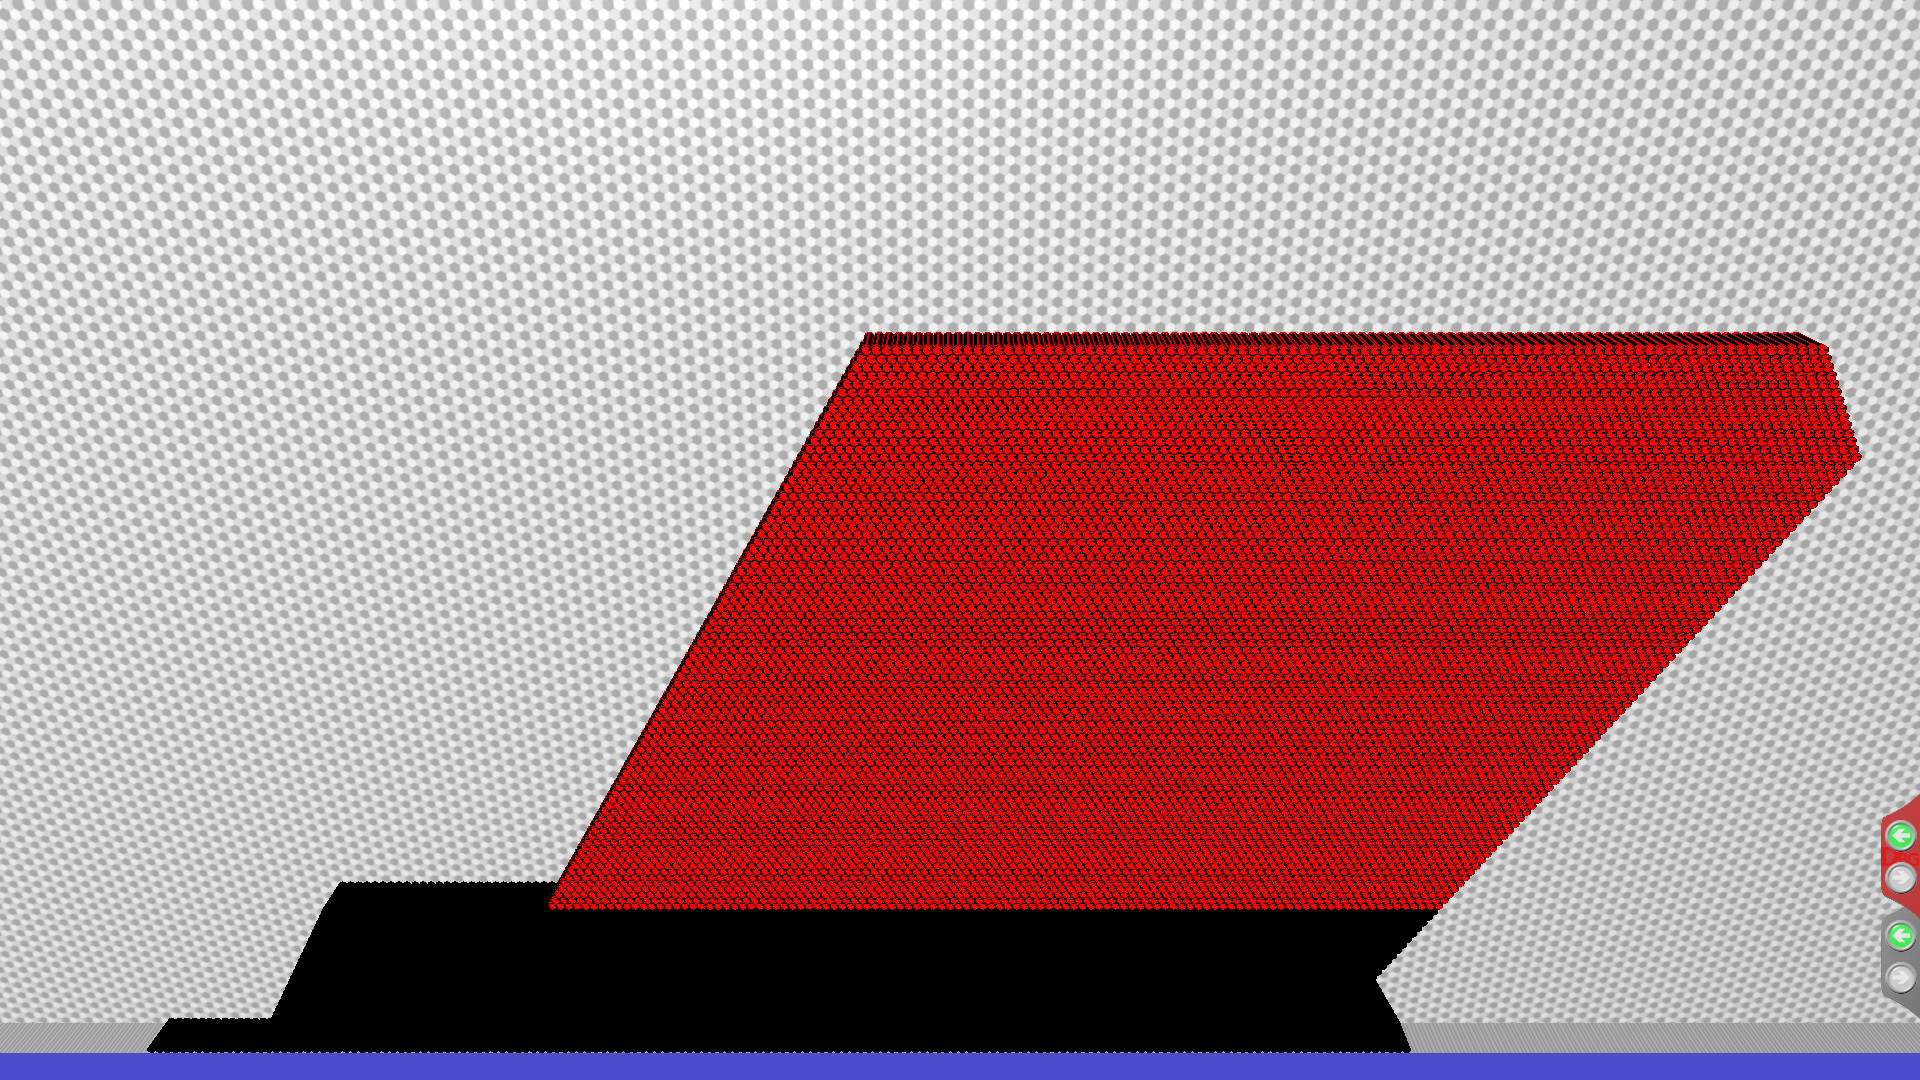
\includegraphics[width=\mySubfigureWidth,height=\mySubfigureHeight]{images/reconfiguration/flag-12407.png}\\
			a) Car (9,644 Catoms). & b) Flag (12,047 Catoms).\\
			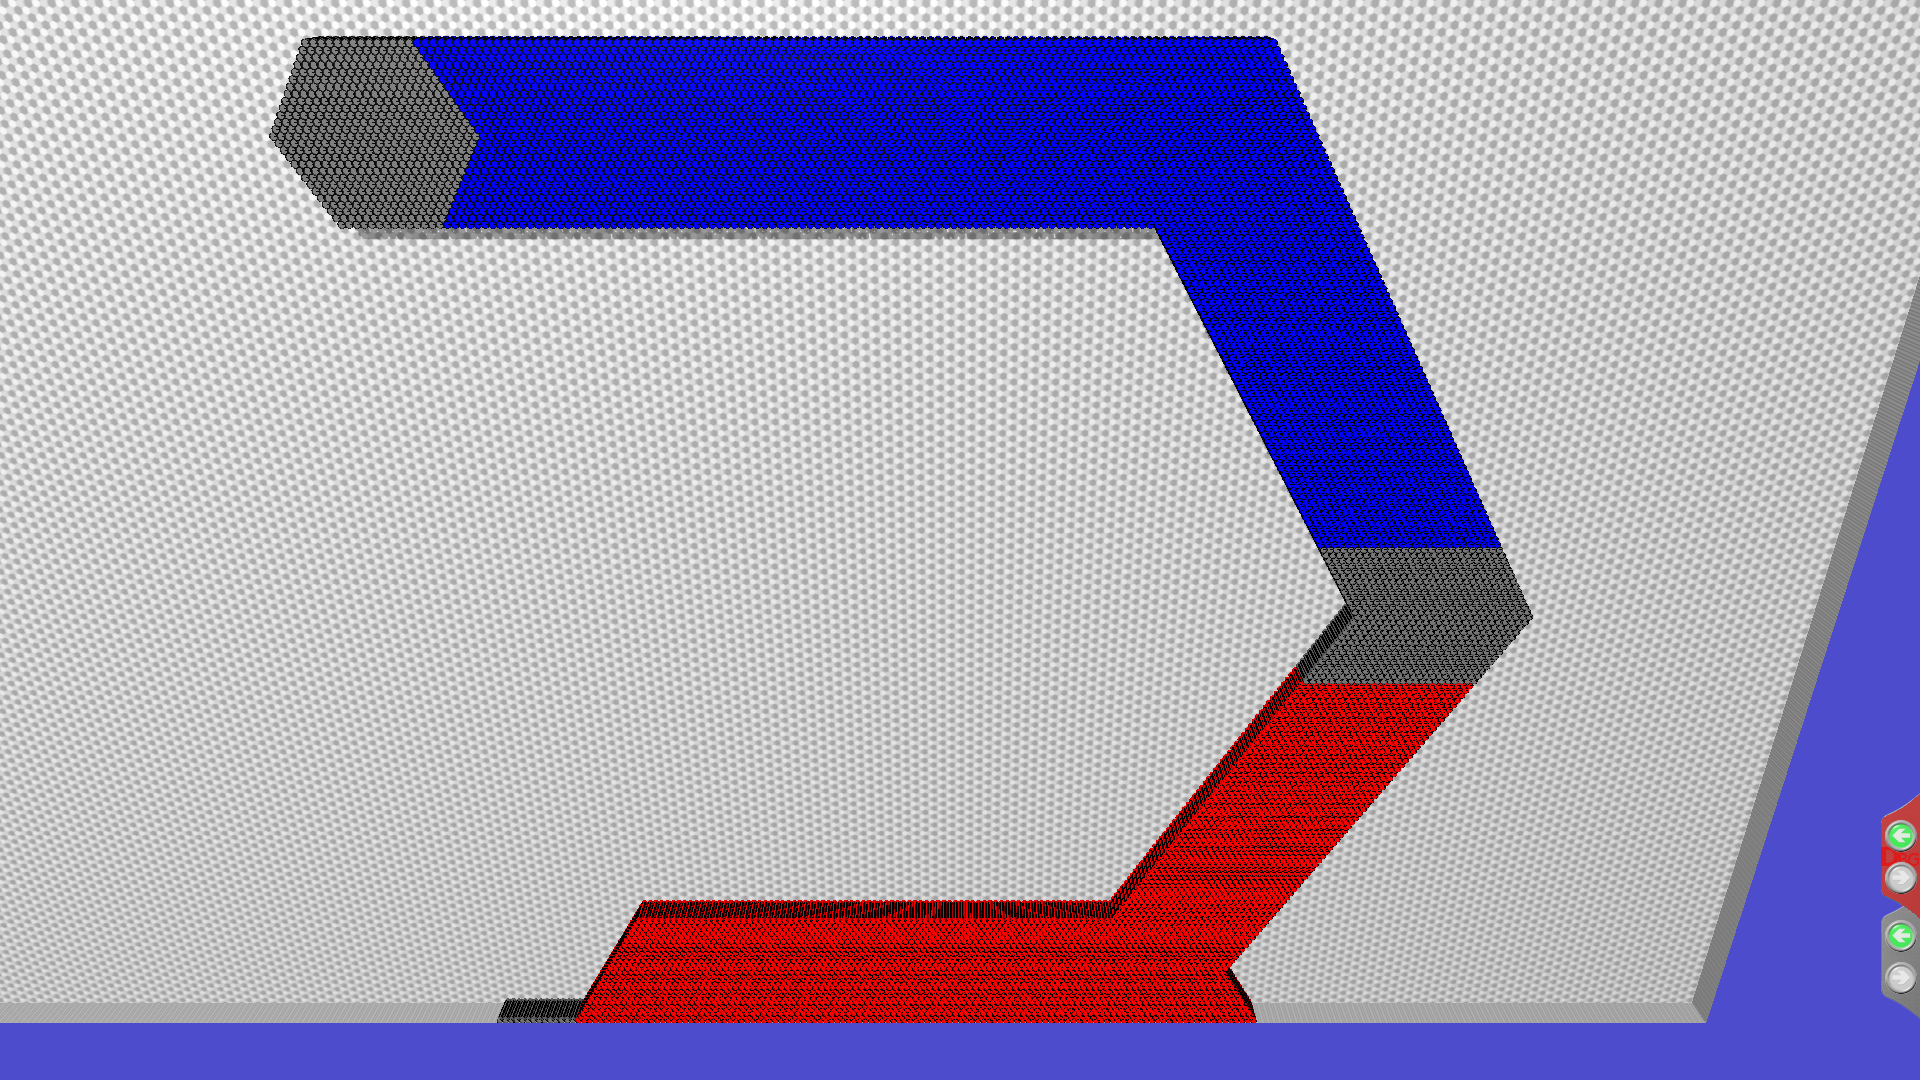
\includegraphics[width=\mySubfigureWidth,height=\mySubfigureHeight]{images/reconfiguration/magnet-10220.png} &
			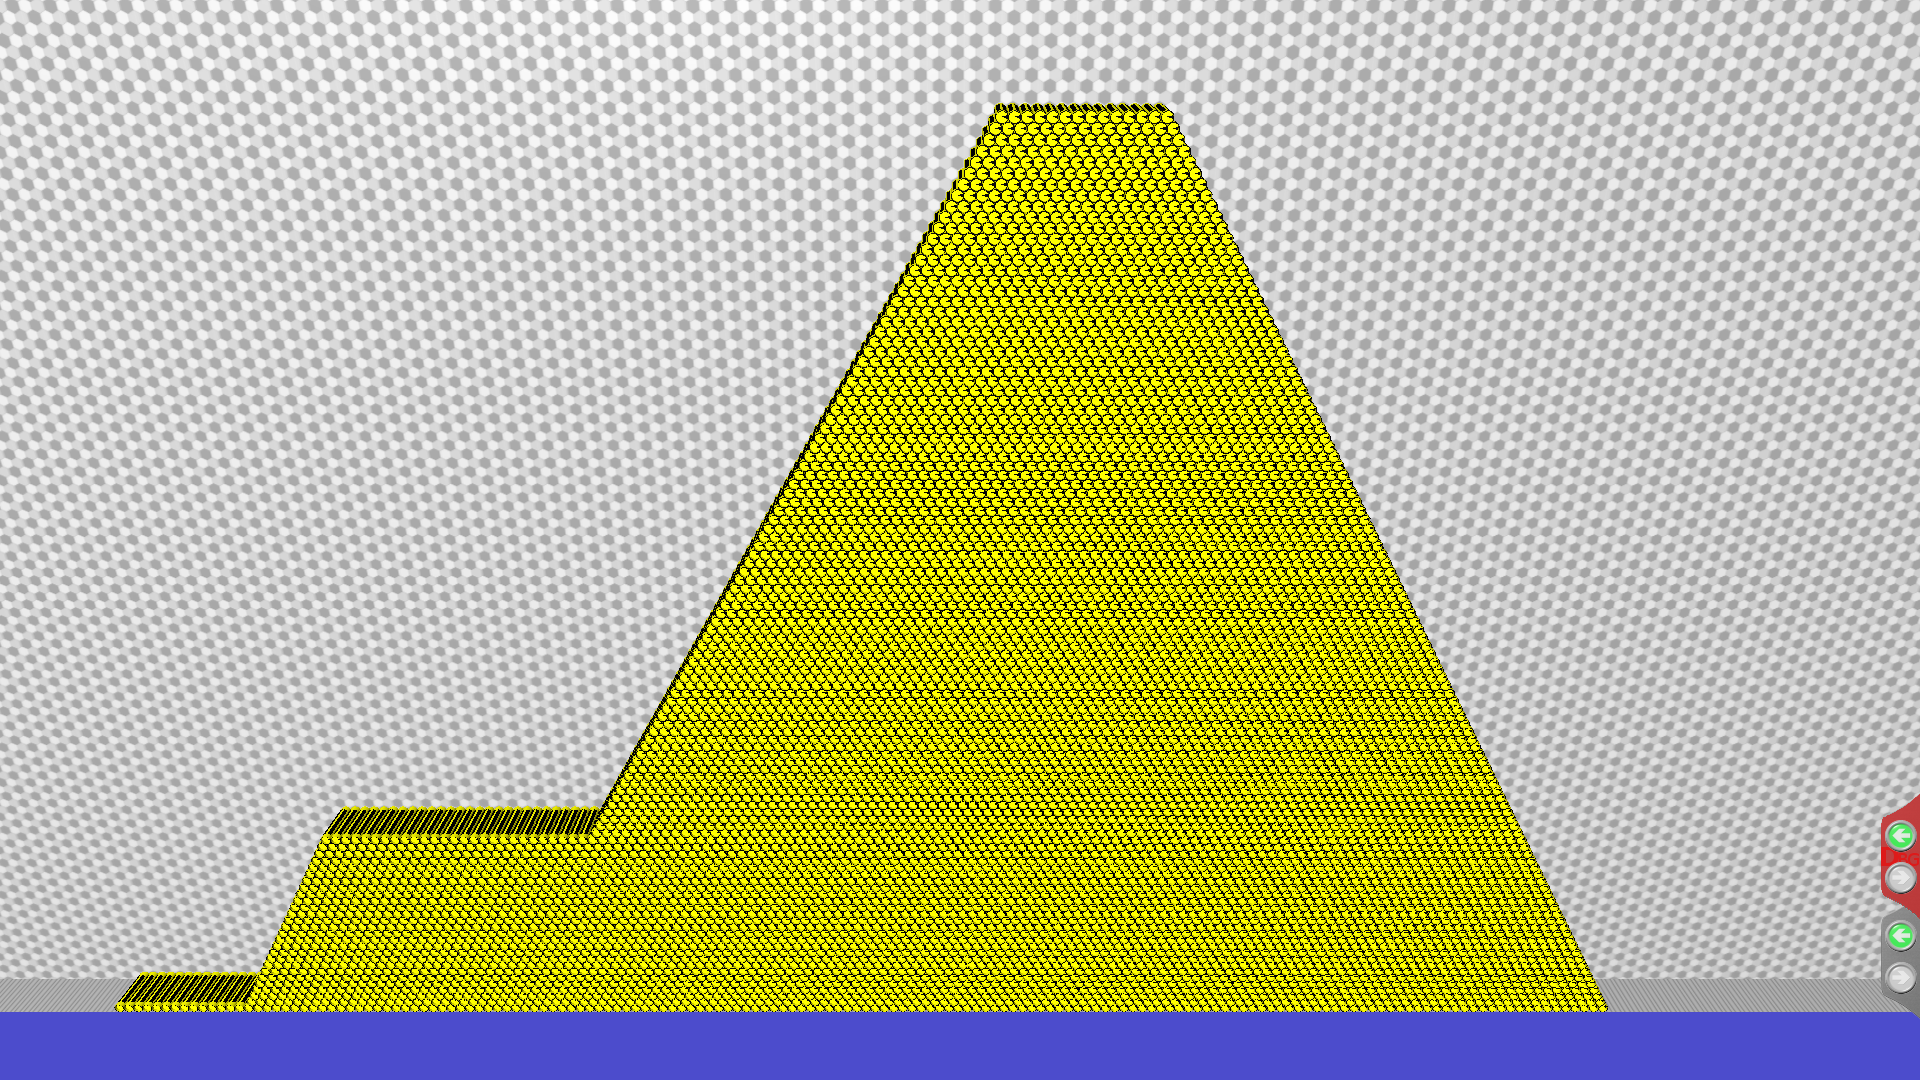
\includegraphics[width=\mySubfigureWidth,height=\mySubfigureHeight]{images/reconfiguration/pyramid-8033.png} \\
			c) Magnet (10,220 Catoms). & d) Pyramid (8,033 Catoms).\\
		\end{tabular}
		\caption{Screenshots of VisibleSim at the end of the simulation of C2SR with different kinds of goal shapes composed of about 10,000 2D Catoms.\label{fig:reconfiguration:shapes}}
	\end{figure}
}

\subsection{Communication Evaluation}

%https://moodle.umons.ac.be/pluginfile.php/69415/mod_resource/content/1/theorie_TPGraphique_erreur.pdf

Figure~\ref{fig:reconfiguration:message} shows the total number of messages sent during the execution of C2SR according to the size of the goal shape. For the shapes we considered, the number of messages seems to depend on the size of the goal configuration and not on the actual shape of the arrangement. Moreover, the standard deviation is very small, so small that it is not visible in the figure. Thus, for a goal shape of a given size, C2SR always sends approximately the same number of messages. Furthermore, as shown in Figure~\ref{fig:reconfiguration:message} by the curve of best fit $y(x) = 20.29x^{1.53}$, this number of messages is highly predictable and increases polynomially with the size of the goal shape.

\begin{figure}[!h]
	\centering
	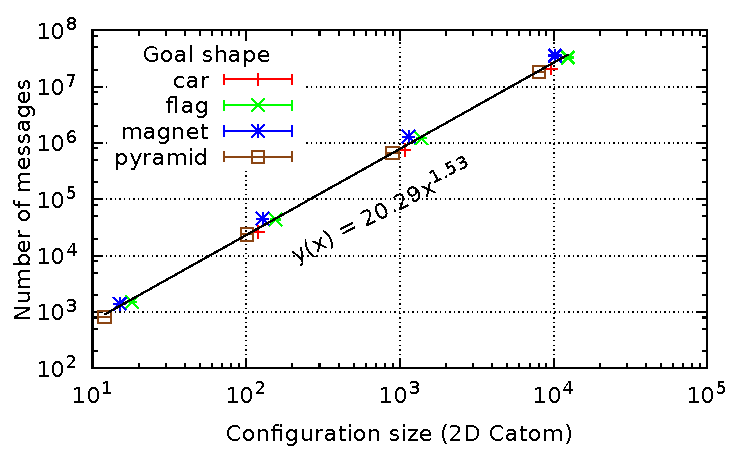
\includegraphics[width=0.7\linewidth]{images/reconfiguration/graphs/message}
	\caption{Average total number of messages ($\pm$~standard deviation) sent in C2SR versus the size of the system for different goal shapes.}
	\label{fig:reconfiguration:message}
\end{figure}

Figure~\ref{fig:reconfiguration:message-individual} indicates that a few modules tend to send a lot more
messages than the other modules. Intuitively, modules that stay at the boundary between $\mathcal{I}$ and $\mathcal{G}$ are communication hotspots because many modules have to communicate with them before rolling over them in order to reach $\mathcal{G}$ (see Figure~\ref{fig:reconfiguration:parallelism}).

\begin{figure}[!h]
	\centering
	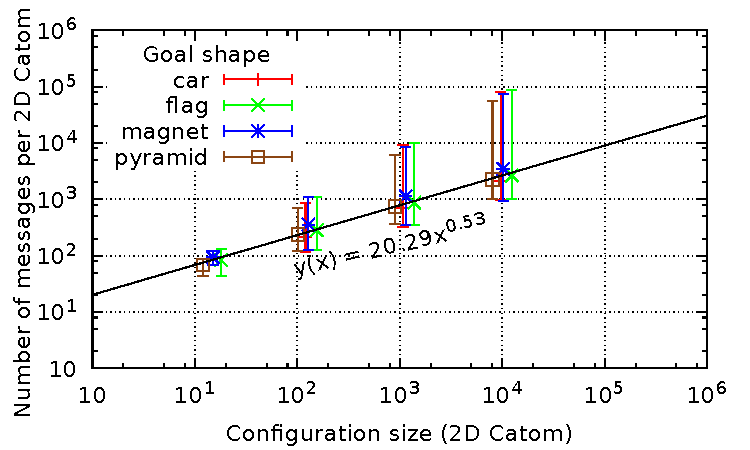
\includegraphics[width=0.7\linewidth]{images/reconfiguration/graphs/message-individual}
	\caption{Average number of messages sent per 2D Catom ($\pm$~min/max) during the execution of C2SR versus the size of the system for different goal shapes.}
	\label{fig:reconfiguration:message-individual}
\end{figure}

Figure~\ref{fig:reconfiguration:queue} shows the maximum message queue size reached by the modules during the execution of C2SR, taking into account both the incoming and the outgoing messages. The maximum message queue size is constant and equal to two, regardless of the shape of the goal configuration and regardless of its size. We recall that messages generated by C2SR have a small and constant size. As a consequence, the traffic generated by C2SR is well controlled and modules do not require a lot of memory space to store incoming and outgoing messages.

Figure~\ref{fig:reconfiguration:hop} shows the average number of hops traveled by the packets during the execution of C2SR. The average and the maximum number of hops traveled by the packets is small and relatively constant, regardless of the shape of the goal configuration and regardless of its size. This confirms that C2SR only involves local interactions, as stated in the previous section.

\begin{figure}[!h]
	\centering
	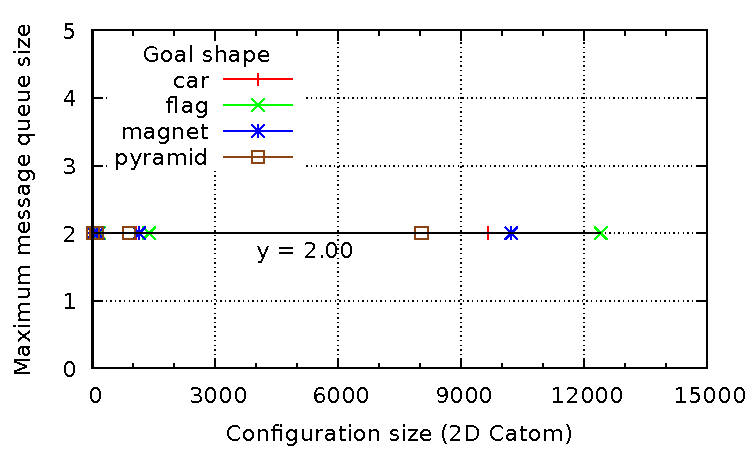
\includegraphics[width=0.7\linewidth]{images/reconfiguration/graphs/queue}
	\caption{Maximum message queue size (incoming and outgoing messages) reached by any node  versus the size of the system during the execution of C2SR.}
	\label{fig:reconfiguration:queue}
\end{figure}

\begin{figure}[!h]
	\centering
	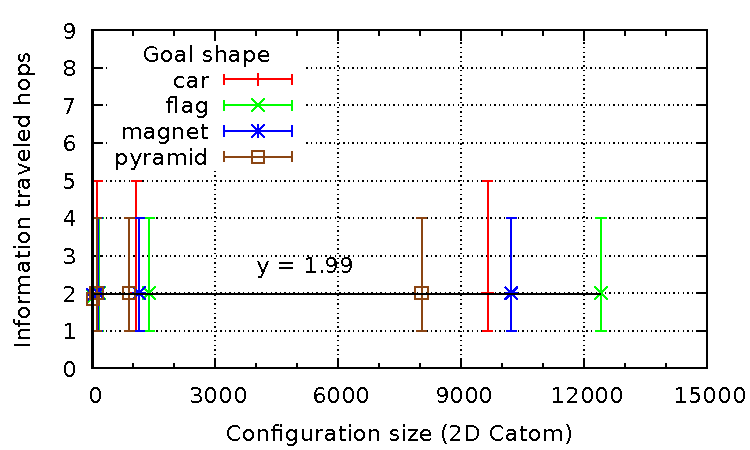
\includegraphics[width=0.7\linewidth]{images/reconfiguration/graphs/hop}
	\caption{Average number of hops traveled by data ($\pm$~min/max) in the execution of C2SR versus the size of the system.}
	\label{fig:reconfiguration:hop}
\end{figure}

\subsection{Motion Efficiency}

Figure~\ref{fig:reconfiguration:cmotion} shows the total number of atomic moves performed during the execution of C2SR according to the size of the system for different goal shapes. Note that this figure is really similar to Figure~\ref{fig:reconfiguration:message}. Here again, the number of atomic moves seems to depend only on the size of the goal configuration and not on the actual shape of the arrangement. As shown in Figure~\ref{fig:reconfiguration:cmotion} by the curve of best fit $y(x) = 2.09x^{1.53}$, the number of atomic moves is highly predictable and increases polynomially with the size of the goal shape. Notice that the number of messages is approximately equal to ten times the number of moves (see Figures~\ref{fig:reconfiguration:message} and~\ref{fig:reconfiguration:cmotion}). Thus, an atomic move requires on average 10 messages.

As shown in Figure~\ref{fig:reconfiguration:parallelism}, many modules can move concurrently during the execution of C2SR. Thus, although the self-reconfiguration process may require many atomic moves, it remains reasonably time-efficient, as shown in the next subsection.

\begin{figure}[!h]
	\centering
	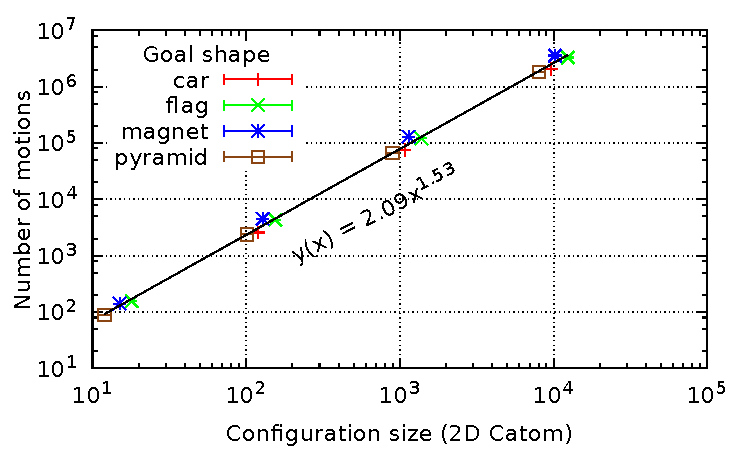
\includegraphics[width=0.7\linewidth]{images/reconfiguration/graphs/motion}
	\caption{Average total number of atomic moves ($\pm$~standard deviation) versus the size of the system for different goal shapes.}
	\label{fig:reconfiguration:cmotion}
\end{figure}

\begin{figure}[!h]
	\centering
	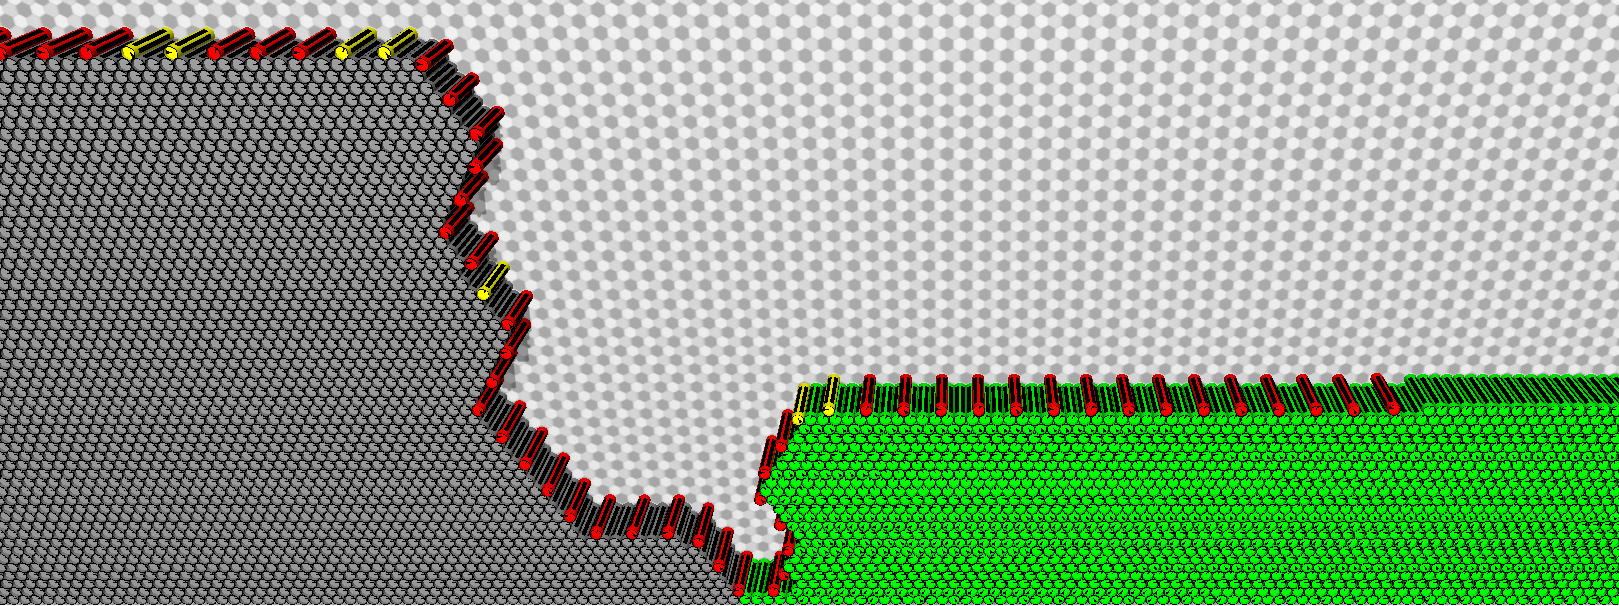
\includegraphics[width=0.7\linewidth]{images/reconfiguration/parallelism}
	\caption{Screenshot of VisibleSim during a self-reconfiguration process with C2SR. Modules in the stream progress by rotating CW. Blocked modules are in gray, waiting ones in yellow, moving ones in red and modules that have converged are in green.}
	\label{fig:reconfiguration:parallelism}
\end{figure}

\subsection{Execution Time Efficiency}

% temps (sec) = a*(#module) + b

% Rscript fit.r ../results-2/car/summary.out
%Coefficients:
%Estimate Std. Error  t value Pr(>|t|)    
%(Intercept) 4.894878   4.151705    1.179  0.44782    
%x           1.047386   0.000741 1413.454  0.00045 ***

% Rscript fit.r ../results-2/pyramid/summary.out 
%Coefficients:
%Estimate Std. Error  t value Pr(>|t|)    
%(Intercept) 3.788747   2.562625    1.478    0.277    
%x           1.028214   0.000634 1621.681  3.8e-07 ***

% Rscript fit.r ../results-2/square/summary.out
%Coefficients:
%Estimate Std. Error  t value Pr(>|t|)    
%(Intercept) 3.9510396  2.6566164    1.487    0.275    
%x           1.0264813  0.0004256 2411.963 1.72e-07 ***

Figure~\ref{fig:reconfiguration:time} shows the average simulated time of C2SR execution according to the size of the system. For the different goal shapes we considered, this time seems to depend only on the size of the configuration and not on the actual shape of the arrangement. Moreover, the standard deviation is very small and not visible in the figure. Thus, for a goal shape of a given size, C2SR always approximately lasts for the same duration. As shown in Figure~\ref{fig:reconfiguration:time} by the curve of best fit $y(x) = 0.017 x + 0.149$, the simulated time is highly predictable and increases linearly with the size of the goal shape. The slope of the line gives the reconfiguration speed: C2SR fills, on average, $\frac{1}{0.017} \approx  59$ goal cells per minute, i.e., approximately 1 cell per second. Note that, in these experiments, the reconfiguration speed is independent of the goal shape.

\begin{figure}[!h]
	\centering
	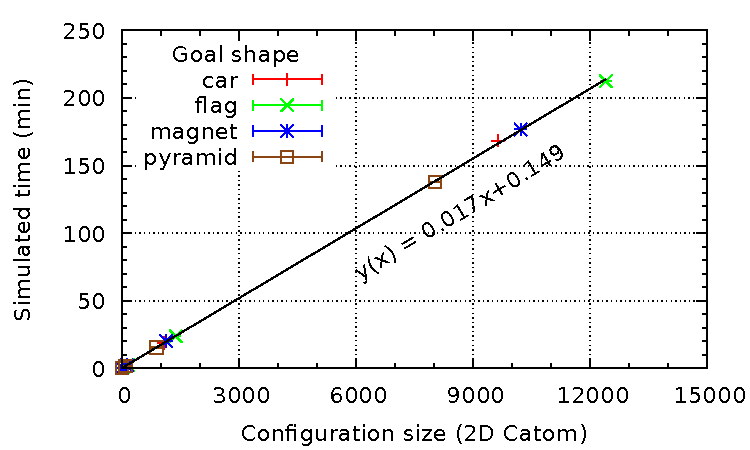
\includegraphics[width=0.7\linewidth]{images/reconfiguration/graphs/time}
	\caption{Average C2SR simulated time ($\pm$~standard deviation) versus the size of the system for different goal shapes.}
	\label{fig:reconfiguration:time}
\end{figure}

Figure~\ref{fig:reconfiguration:rate} shows the average simulated time of the C2SR execution according to the average communication bitrate for the two different motion speeds supported by the 2D Catoms. We consider the usual bitrates of serial communications. We conducted this experiment for the car goal shape composed of 1,073 modules. Until 38.9~kbit/s, the self-reconfiguration process becomes much faster, as the average communication bitrate increases. Beyond 38.9~kbit/s, the self-reconfiguration speed increases less quickly and tends to stabilize.

\begin{figure}[!h]
	\centering
	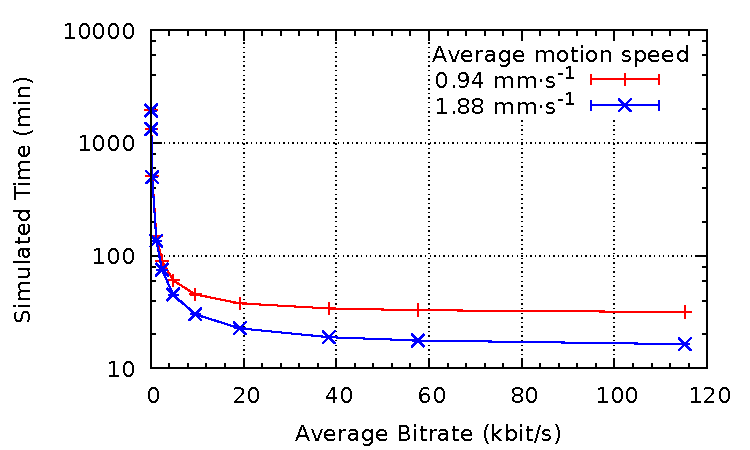
\includegraphics[width=0.7\linewidth]{images/reconfiguration/graphs/rate}
	\caption{Average C2SR simulated time ($\pm$ standard deviation) versus the communication bitrate (random initial configuration into the car of 1,073 2D Catoms).}
	\label{fig:reconfiguration:rate}
\end{figure}

\section{Conclusion}
\label{section:reconfiguration:conclusion}

In this chapter, we proposed the Cylindrical-Catoms Self-Reconfiguration (C2SR) algorithm, a parallel, asynchronous and fully decentralized distributed algorithm to self-reconfigure a lattice-based \gls{msr} from an initial shape into a goal one. We evaluated our algorithm using simulations on ensembles with up to 10,020 Catoms. The results show that C2SR has nice properties.